\chapter{The Computation History Method}

\begin{remark}[Remember]
    To prove some language B is undecidable, show that \(A_{TM}\) (or any known decidable language) is reducible to B. 
\end{remark}

\section{Computation History}
\begin{definition}[TM configuration]
    A \underline{configuration} of a TM is a triple \((q, p, t)\) where
    \begin{itemize}
        \item \(q\) = the state,
        \item \(p\) = the head position,
        \item \(t\) = tape contents   
    \end{itemize} 
    representing a snapshot of the TM at a point in time.
\end{definition}

\begin{remark}[Encode a configuration]
    Encode configuration \((p, q, t)\) as string \(t_1 q t_2\)  where \(t = t_1t_2\) and the head position is on the first symbol of \(t_2\).   
    \begin{example}
        Configuration: \((q_3, 6, aaaaaabbbbb)\) 

        Encoding as string: \(aaaaaq_3abbbbb\) 
    \end{example}
\end{remark}

\begin{definition}[TM Computation History]
    An \underline{(accepting) computation history} for TM \(M\) on input \(w\) is a sequence of configurations \(C_1, C_2, \cdots, C_{accept}\) that \(M\) enters until it accepts.   
    \begin{intuition}
        It's like the log of the execution of the machine.
    \end{intuition}
\end{definition}

\begin{remark}[Encode a computation history]
    Encode a computation history as \(C_1\#C_2\#\cdots\#C_{accept}\) 
    where each configuration is encoded as a string.
\end{remark}


\section{Linearly Bounded Automata}

\begin{definition}[Linealy Bounded Automata(LBA)]
A linearly bounded automata (LBA) is a 1-tape TM that cannot move its head off the input portion of the tape.
\end{definition}

\begin{remark}
    Tape size adjusts to the length of input.
\end{remark}

\begin{figure}[H]
    \centering
    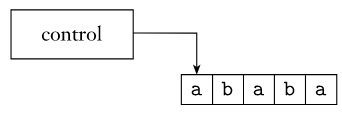
\includegraphics[width=0.4\textwidth]{f5.7.jpg}
    \caption{Schematic of an LBA}
\end{figure}

\begin{theorem}
    Let \(A_{LBA} = \{ \langle B, w \rangle | LBA\; B \; accepts \; w\} \) 

    \(A_{LBA}\) is decidable. 
\end{theorem}
\begin{proof}
    (idea) If \(B\) on \(w\) runs for long, it must be cycling. 

    \begin{remark}
        For inputs of length \(n\), an LBA  can have only \(|Q| \times n \times |\Gamma|^n\) different configurations. 

        Therefore, if an LBA runs for longer, it must repeat some configurations and thus will never halt.
    \end{remark}
\end{proof}

\begin{theorem}
    Let \(E_{LBA}\) = \{ \(\langle B \rangle\) | \(B\) is an LBA and \(L(B) = \emptyset\)  \} 

    \(E_{LBA}\) is undecidable. 
\end{theorem}
\begin{proof}
    Show \(A_{TM}\) is reducible to \(E_{LBA}\).  

    Assume \(R\) decides \(E_{LBA}\), we can construct a TM \(S\) deciding \(A_{TM}\) (which is contradiction): 

    \(S = \) "on input \(\langle M, w \rangle\)
    \begin{enumerate}
        \item Construct LBA \(B_{M, w}\) which tests whether its input \(x\) is an accepting computation history for \(M\) on \(w\), and only accepts \(x\) if it is.
        \item Use \(R\) to determine whether \(L(B_{M, w}) = \emptyset\).       
        \item Accept if no. Reject if yes."
    \end{enumerate}    

    Why we can construct an LBA \(B_{M, w}\) like that? Because for the LBA, input \(x\) is the content on the tape, the LBA can move its header on the tape and follow this history and verify if it is a valid history of input \(w\).  
\end{proof}


\section{History Method for proving undecidability}

\begin{example}[Hilbert's \(10^{th}\) Problem]
    Recall  \(D = \) \{ \(\langle p \rangle\) | polynomial \(p(x_1, x_2, \cdots, x_k) = 0\) has integer solution\}
\end{example}
\begin{theorem}
    Hilbert's \(10^{th}\) problem: Is \(D\) decidable? No.  
\end{theorem}
\begin{proof}
    Show \(A_{TM}\) is reducible to \(D\).   
\end{proof}

Do toy problem instead which has a similar proof method: PCP. The method is The Computation History Method.

\section{Post Correspondence Problem (PCP)}

\begin{problem}[PCP problem]
    Give a collection of pairs of strings as dominoes:
    
    \[
        P = \{ 
            \begin{bmatrix}
             t_1 \\
             b_1 \\
            \end{bmatrix} 
            ,
            \begin{bmatrix}
             t_2 \\
             b_2 \\
            \end{bmatrix}
            , 
            \cdots
            ,
            \begin{bmatrix}
             t_k \\
             b_k \\
            \end{bmatrix}
        \} 
    \]

    A \underline{match} is a finite sequence of dominoes in \(P\) (repeats allowed) where the concatenation of the \(t's\) = the concatenation of the \(b's\). 

    \begin{example}
        Match = \(
        \begin{bmatrix}t_{i_1} \\b_{i_1} \end{bmatrix}
        \begin{bmatrix}t_{i_2} \\b_{i_2} \end{bmatrix}
        \cdots
        \begin{bmatrix}t_{i_3} \\b_{i_3} \end{bmatrix}
        \) 
        where \(t_{i_1}t_{i_2}\cdots t_{i_l} = b_{i_1}b_{i_2}\cdots b_{i_l}\) 
    \end{example}

    \begin{example}
        \[
            P= \{ 
            \begin{bmatrix}ab \\ aba \end{bmatrix}
            \begin{bmatrix}aa \\ aba \end{bmatrix}
            \begin{bmatrix}ba \\ aa \end{bmatrix}
            \begin{bmatrix}abab \\ b \end{bmatrix}
            \} 
        \]


        Match:
        \begin{figure}[H]
            \centering
            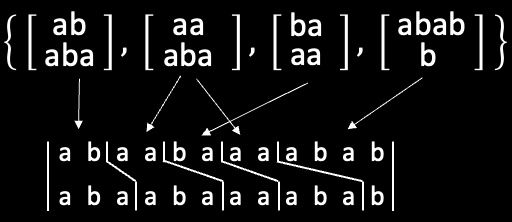
\includegraphics[width=0.4\textwidth]{l10.1.jpg}
            \caption{A match}
        \end{figure}
    \end{example}

    Problem: Given \(P\), is there a match?
\end{problem}


\begin{theorem}[PCP problem]
    The above problem is undecidable. (there's no problem to solve the problem)

    Formalize the problem:

    Let \(PCP = \) \{ \(\langle P \rangle\)| \(P\) has a match\}
\end{theorem}
\begin{proof}[PCP problem]
    IDEA: Show \(A_{TM}\) is reducible to \(PCP\).  

    The main technique is reduction from \(A_{TM}\) via accepting computation histories. 

    How to do it? We try to make a connection that for any TM \(M\) and input \(w\), we can construct an instance P:

    \fbox{
    P has a match \(\implies\) An accepting computation history for \(M\) on \(w\).  
    }

    We will give some assumptions to make the proof simpler, and we can eliminate those assumptions later.

    \begin{problem}[Modified PCP (MPCP)]
        We modify the PCP to require that a match starts with the first domino, \(\begin{bmatrix}
                t_1 \\
                b_1 
        \end{bmatrix} \). 


        \(MPCP\) = \{ \(\langle P \rangle \) | \(P\) is an instance of the PCP with a match that starts with the first domino\} 
    \end{problem}
    \begin{proof}
        We are given \(M\) and \(w\), we're trying to make a set of dominoes, where a match will be a computation history for \(M\) on \(w\).    

        How we make our dominoes?

        \textbf{Part 1}: Starting domino:
        \[
            \begin{bmatrix}
                 u_1 \\
                 v_1 \\
            \end{bmatrix}
            = 
            \begin{bmatrix}
                 \# \\
                 \#q_0w_1\cdots w_n\# \\
            \end{bmatrix}
        \] 
    \end{proof}
    \begin{proof}[Cont.]
        \begin{figure}[H]
            \centering
            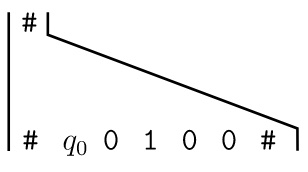
\includegraphics[width=0.2\textwidth]{l10.2-1.jpg}
            \caption{With Part 1 domino}
        \end{figure}


        \textbf{Part 2}: For each \(a, b \in \Gamma\)(alphabet in tape) and \(q, r \in Q\)(states) where our transition function be \(\delta(q, a) = (r, b, R)\)(If the TM in state \(q\), and the head is \(a\), it moves to state \(r\), write \(b\) into it and its head move one step to the right). 
        This information can be captured by domino:
        \[
            \begin{bmatrix}
                q & a  \\
                b & r  \\
            \end{bmatrix}
        \]

        \textbf{Part 3}: For every \(a \in \Gamma\), we put this domino:
        \[
            \begin{bmatrix}
                 a \\
                 a \\
            \end{bmatrix}
        \]  

        \textbf{Part 4}: We also need to have \(\#\), it is not in \(\Gamma\), so I make it different part:
        \[
            \begin{bmatrix}
                 \# \\
                 \# \\
            \end{bmatrix}
        \]
        \begin{figure}[H]
            \centering
            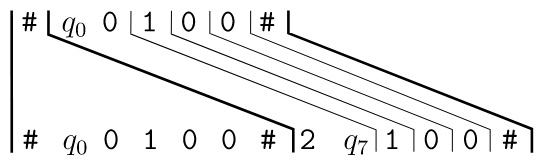
\includegraphics[width=0.4\textwidth]{l10.2-2.jpg}
            \caption{With Part 2, 3, 4 dominoes}
        \end{figure}

        When we're adding more states, the bottom will have \(q_{accept}\), it is done for the perspective of the \(M\); 
        but it is not a match yet! 
        Notice that the bottom is like always a configuration ahead of the top.

        \textbf{Part 5}: To make the match, we add dominoes like these:
        \[
            \begin{bmatrix}
                 a q_{accept} \\
                 q_{accept} \\
            \end{bmatrix}    
            \quad
            \begin{bmatrix}
                 q_{accept} a \\
                 q_{accept} \\
            \end{bmatrix}
        \]

        \begin{figure}[H]
            \centering
            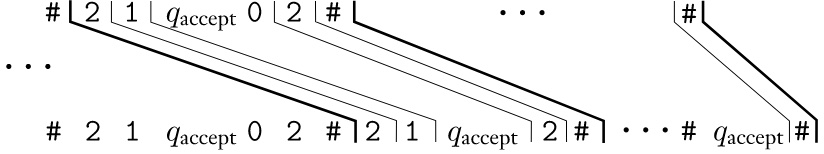
\includegraphics[width=0.6\textwidth]{l10.2-3.jpg}
            \caption{With Part 5 dominoes}
        \end{figure}

        \textbf{Part 6}: To end, we add:
        \[
            \begin{bmatrix}
                 q_{accept} \# \# \\
                 \# \\
            \end{bmatrix}
        \] 
        \begin{figure}[H]
            \centering
            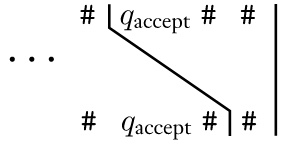
\includegraphics[width=0.2\textwidth]{l10.2-4.jpg}
            \caption{With Part 6 domino}
        \end{figure}
    \end{proof}
    \newpage
    \begin{proof}[Cont.]
        \begin{remark}
            Why we can have consecutive \(\#\)s? Because there are \(\epsilon\).  
        \end{remark}

        Now we assume that TM \(R\) decides \(PCP\).  

        We construct TM \(S\) deciding \(A_{TM}\):

        \(S =\) "on input \(\langle M, w\rangle\)
            \begin{enumerate}
                \item Construct \(PCP\) instance \(P_{M, w}\)(what we have done!) where a match corresponds to a computation history for \(M\) and \(w\).   
                \item Use \(R\) to determine whether \(P_{M, w}\) has a match.  
                \item Accept if yes, Reject if no."
            \end{enumerate}
    \end{proof}
\end{proof}


\begin{theorem}
    Let \(ALL_{CFG} = \)\{ \(\langle G \rangle\) | \(G\) is a CFG and \(L(G) = \Sigma^*\)   \} 

    \(ALL_{CFG}\) is undecidable. 
\end{theorem}
\begin{proof}
    Show \(A_{TM}\) is reducible to \(ALL_{PDA}\) via the computation history method.  

    Assume TM \(R\) decides \(ALL_{PDA}\) and construct TM \(S\) deciding \(A_{TM}\).    

    \(S = \) "On input \(\langle M, w \rangle\) 
    \begin{enumerate}
        \item Construct PDA \(B_{M, w}\) which tests whether its input \(x\) is an accepting computation history for \(M\) and \(w\), and only accepts \(x\) if it is NOT
        \item Use \(R\) to determine whether \(L(B_{M, w}) = \Sigma^*\) 
        \item Accept if no, Reject if yes."      
    \end{enumerate}
\end{proof}